\documentclass[11pt]{article}
\usepackage{cse103}
\def\title{HW 3}

% use the tikz package to draw automata
\usepackage{tikz}
\usetikzlibrary{arrows,positioning,automata}

\begin{document}
\maketitle

\section*{Due October 20 at 11:59pm}

\textbf{(6 questions, 230 points total)}

\begin{qunlist}


\q{40}{Conversion of NFAs to DFAs}\\
Consider the following NFA $N$ over the alphabet $\Sigma = \{a,b\}$:

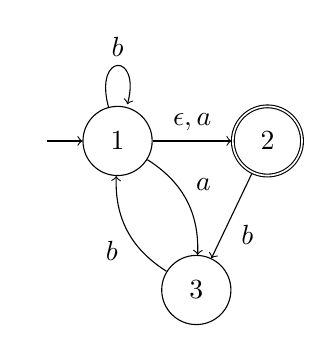
\begin{tikzpicture}
\node[state, initial, initial text=] (s1) {$1$};
\node[state, accepting, right= of s1] (s2) {$2$};
\node[state, below= of s1, xshift=1cm] (s3) {$3$};

\path[->]
  (s1) edge[loop above] node[above] {$b$} (s1)
  (s1) edge node[above] {$\epsilon, a$} (s2)
  (s1) edge[bend left] node[above right] {$a$} (s3)
  (s2) edge node[below right] {$b$} (s3)
  (s3) edge[bend left] node[below left] {$b$} (s1);
\end{tikzpicture}

\begin{qparts}
\item \emph{(30 pts.)}
Use the construction we described in class to build a DFA $D$ equivalent to $N$.
Draw $D$ as a graph, omitting any states which are not reachable from the start state.

\item \emph{(10 pts.)}
Even dropping unreachable states, $D$ is not the smallest DFA equivalent to $N$.
Draw another DFA $D'$ which is equivalent to $N$ and has as few states as possible (you don't need to prove this).
\end{qparts}

\newpage

\q{45}{Intersecting automata}\\
We showed in class that if $L_1$ and $L_2$ are regular languages, then so is $L_1 \cap L_2$, since $L_1 \cap L_2 = \overline{\overline{L_1} \cup \overline{L_2}}$ and regular languages are closed under union and complement.
\begin{qparts}
\item \emph{(10 pts.)}
Suppose we have DFAs $D_1$ and $D_2$ for $L_1$ and $L_2$ with $n$ and $m$ states respectively.
Describe the sequence of transformations you would use to turn these into a DFA for $\overline{\overline{L_1} \cup \overline{L_2}}$ (and so for $L_1 \cap L_2$), stating after each step how many states the resulting automaton has.

\item \emph{(35 pts.)}
A more direct way to build a DFA for $L_1 \cap L_2$ is the \emph{product construction}.
The idea is to run the DFAs for $L_1$ and $L_2$ in parallel: each time we read an input symbol, we update the states of both automata, and we accept only if both automata end in an accepting state.
To simulate running both automata in parallel, we use a DFA whose states are labeled by \emph{pairs} of states, one from each automaton; then the transitions are defined by updating each component of the pair independently.
Formally, starting with DFAs $D_1 = (Q_1, \Sigma, \delta_1, q_{01}, F_1)$ and $D_2 = (Q_2, \Sigma, \delta_2, q_{02}, F_2)$, the \emph{product automaton} $D$ is defined as follows:
\begin{itemize}
\item $Q = Q_1 \times Q_2$ \quad (all pairs with a state from $Q_1$ and a state from $Q_2$)
\item $\delta((q_1, q_2), s) = (\delta_1(q_1, s), \delta_2(q_2, s))$
\item $q_0 = (q_{01}, q_{02})$
\item $F = \{ (q_1, q_2) \in Q \st q_1 \in F_1 \text{ and } q_2 \in F_2 \}$.
\end{itemize}

Prove that the product construction works: $L(D) = L(D_1) \cap L(D_2)$.\\
(\emph{Hint:} Compare the extended transition functions of $D$, $D_1$, and $D_2$.)
\end{qparts}

\newpage


\q{35}{Reading regular expressions}\\
For each of the following pairs of regular expressions over $\Sigma = \{a, b, c\}$, state whether their languages are equal ($=$), one is a proper subset of the other ($\subset$), or if they are incomparable.
If $L(R_1) \subset L(R_2)$, give an example of a string in $L(R_2)$ that is not in $L(R_1)$, or vice versa if $L(R_2) \subset L(R_1)$; if the languages are incomparable, give an example string from each language that is not in the other.

\begin{qparts}
\item
$R_1 = a^* b^*$ \\
$R_2 = (a^* b^*)^*$

\item
$R_1 = (a | b | c)^*$ \\
$R_2 = (a^* b^* c^*)^*$

\item
$R_1 = c^* c$ \\
$R_2 = (cc)^* \; | \; c(cc)^*$

\item
$R_1 = c^* (a | b | \epsilon) c^*$ \\
$R_2 = c^* a c^* \; | \; c^* b c^*$

\item
$R_1 = \emptyset b \; | \; a a^*$ \\
$R_2 = a^*$
\end{qparts}

\newpage

\q{45}{Writing regular expressions}\\
Write regular expressions for the following languages over $\Sigma = \{a,b,c,\dots,z\}$:

\begin{qparts}
\item
Strings containing the substring $dog$ followed eventually (not necessarily immediately) by either the substring $cat$ or the substring $rat$.

\item
Strings containing both $x$ and $y$, where the first $x$ is followed by a $y$ within 3 symbols (e.g. $xy$ and $xzzy$ are fine but not $xzzzy$).

\item
Strings containing an even number of $z$s.
\end{qparts}

\newpage

\q{20}{Converting a regular expression to an NFA}\\
Convert the regular expression $(a \;|\; c\Sigma)^* a$ to an equivalent NFA.

\newpage

\q{45}{Properties of regular languages}\\
Prove each of the following facts about regular languages.
Give a short argument using results from class and/or simple constructions of automata or regular expressions (no need for proofs by induction).

\begin{qparts}
\item
Every finite language (i.e., a language consisting of finitely many strings) is regular.

\item
If $I$, $T$, and $E$ are regular languages over $\Sigma$, then so is the language
\[
\textsc{If-Then-Else}(I, T, E) = \{ x y \in \Sigma^* \st x \in I \rightarrow y \in T \text { and } x \not \in I \rightarrow y \in E \} .
\]

\item
If $s \in \Sigma$, and $L$ and $R$ are regular languages over $\Sigma$, then so is the language $\textsc{Replace}(L, s, R)$ obtained by taking every string in $L$ and replacing each occurrence of the symbol $s$ by any string in $R$.

(For example, if $L = \{ a, aa, aba \}$, $s = a$, and $R = \{ c, dd \}$, then $\textsc{Replace}(L, s, R)$ is \\$\{ c, dd, cc, cdd, ddc, dddd, cbc, cbdd, ddbc, ddbdd \}$.)
\end{qparts}


\end{qunlist}
\end{document}